\subsection[Attribute]{Embedded Systems Attributes}

\begin{frame}
  \frametitle{What is an Embedded System?}
  \begin{itemize}
    \item A system with restrictions
  \end{itemize}
\end{frame}

\begin{frame}
  \frametitle{What is an Embedded System?}
  \begin{itemize}
    \item A system with restrictions
    \item Designed for a {\bf specific purpose}
  \end{itemize}
\end{frame}

\begin{frame}
  \frametitle{Attributes}
  \begin{itemize}
    \item {\bf CPU}
  \end{itemize}
\end{frame}

\begin{frame}
  \frametitle{CPU}
  \begin{itemize}
    \item $\mu$-controllers and $\mu$-processors
  \end{itemize}
\end{frame}

\begin{frame}
  \frametitle{CPU}
  \begin{itemize}
    \item $\mu$-controllers and $\mu$-processors
    \item Clock Speed ($\lesssim 2.5 GHz$)
  \end{itemize}
\end{frame}

\begin{frame}
  \frametitle{CPU}
  \begin{itemize}
    \item $\mu$-controllers and $\mu$-processors
    \item Clock Speed ($\lesssim 2.5 GHz$)
    \item HW Parallelism (pipelining, SIMD, etc.)
  \end{itemize}
\end{frame}

\begin{frame}
  \frametitle{CPU}
  \begin{itemize}
    \item $\mu$-controllers and $\mu$-processors
    \item Clock Speed ($\lesssim 2.5 GHz$)
    \item HW Parallelism (pipelining, SIMD, etc.)
    \item Floating-Point Unit
  \end{itemize}
\end{frame}

\begin{frame}
  \frametitle{ARM$\textregistered$ Cortex$\textregistered$-A9}
  \begin{center}
    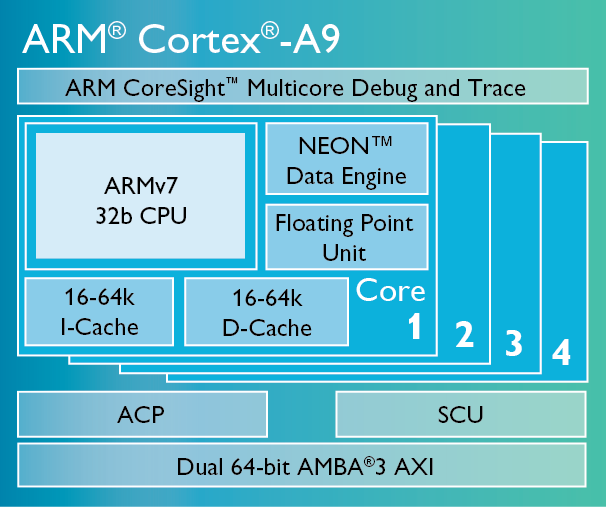
\includegraphics[width=0.7\textwidth]{slides/te5009-embedded-systems-attributes/Cortex-A9-chip-diagram-LG.png}
  \end{center}
\end{frame}

\begin{frame}
  \frametitle{Attributes}
  \begin{itemize}
    \item CPU
    \item {\bf Integration Level}
  \end{itemize}
\end{frame}

\begin{frame}
  \frametitle{Integration Level}
  \begin{itemize}
    \item Highly Integrated Processors called {\it System on Chip} ({\bf SoC})
  \end{itemize}
\end{frame}


\begin{frame}
\frametitle{Freescale i.MX SoC Family}
  \begin{itemize}
    \item
     \url{http://cache.freescale.com/files/32bit/doc/brochure/FLYRIMXPRDCMPR.pdf} 
  \end{itemize}
\end{frame}

\begin{frame}
  \frametitle{Attributes}
  \begin{itemize}
    \item CPU
    \item Integration Level
    \item {\bf Power Consumption}
  \end{itemize}
\end{frame}

\begin{frame}
  \frametitle{Attributes}
  \begin{itemize}
    \item CPU
    \item Integration Level
    \item Power Consumption
    \item {\bf Boards}
  \end{itemize}
\end{frame}

\begin{frame}
  \frametitle{Boards: Freescale i.MX SabreSD}
  \begin{center}
    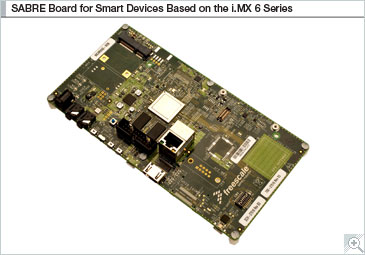
\includegraphics[width=0.5\textwidth]{slides/te5009-embedded-systems-attributes/RDIMX6SABREBRD_BDTN.jpg}
  \end{center}
\end{frame}

\begin{frame}
  \frametitle{Boards: Solid-Run i.MX Humming Board}
  \begin{center}
    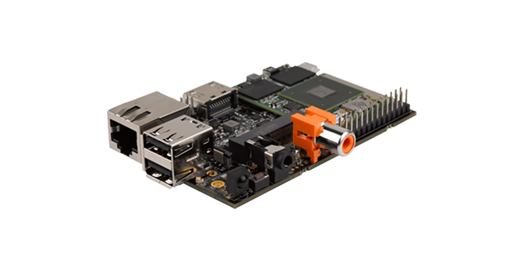
\includegraphics[width=0.7\textwidth]{common/Img_HummingBoard_2.png}
  \end{center}
\end{frame}

\begin{frame}
  \frametitle{Attributes}
  \begin{itemize}
    \item CPU
    \item Integration Level
    \item Power Consumption
    \item Boards
    \item {\bf Expansion}
  \end{itemize}
\end{frame}

\begin{frame}
  \frametitle{Expansion}
  \begin{itemize}
    \item Most of the times there is {\bf no} way to {\bf HW} expand
    \item Should be based on {\bf new SW} features
  \end{itemize}
\end{frame}

\begin{frame}
  \frametitle{Attributes}
  \begin{itemize}
    \item CPU
    \item Integration Level
    \item Power Consumption
    \item Boards
    \item Expansion
    \item {\bf Application Specific HW}
  \end{itemize}
\end{frame}
\begin{frame}

\frametitle{Application Specific HW}
  \begin{itemize}
    \item These days SW features {\bf dictates} HW requirements
  \end{itemize}
\end{frame}

\begin{frame}
  \frametitle{GPU \& VPU \& IPU on i.MX6Q}
  \begin{center}
    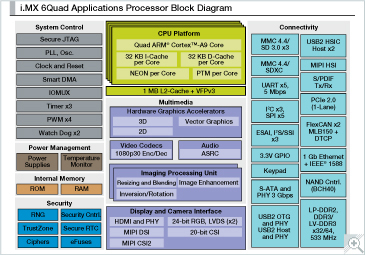
\includegraphics[width=0.5\textwidth]{slides/te5009-embedded-systems-attributes/IMX6Q_BD_TN.jpg}
  \end{center}
\end{frame}

\begin{frame}
  \frametitle{Attributes}
  \begin{itemize}
    \item CPU
    \item Integration Level
    \item Power Consumption
    \item Boards
    \item Expansion
    \item Application Specific HW
    \item {\bf Certifications}
  \end{itemize}
\end{frame}

\begin{frame}
  \frametitle{Attributes}
  \begin{itemize}
    \item CPU
    \item Integration Level
    \item Power Consumption
    \item Boards
    \item Expansion
    \item Application Specific HW
    \item Certifications
    \item {\bf Reliability/Availability}
  \end{itemize}
\end{frame}

\begin{frame}
  \frametitle{Attributes}
  \begin{itemize}
    \item CPU
    \item Integration Level
    \item Power Consumption
    \item Boards
    \item Expansion
    \item Application Specific HW
    \item Certifications
    \item Reliability/Availability
    \item {\bf User Interfaces}
  \end{itemize}
\end{frame}

\begin{frame}
  \frametitle{User Interfaces}
  \begin{itemize}
    \item {\bf headed}: without display (serial console, simple web interface, etc)
    \item {\bf headless}: with display
  \end{itemize}
\end{frame}

\begin{frame}
  \frametitle{Attributes}
  \begin{itemize}
    \item CPU
    \item Integration Level
    \item Power Consumption
    \item Boards
    \item Expansion
    \item Application Specific HW
    \item Certifications
    \item Reliability/Availability
    \item User Interfaces
    \item {\bf Connectivity}
  \end{itemize}
\end{frame}


\begin{frame}
  \frametitle{Attributes}
  \begin{itemize}
    \item CPU
    \item Integration Level
    \item Power Consumption
    \item Boards
    \item Expansion
    \item Application Specific HW
    \item Certifications
    \item Reliability/Availability
    \item User Interfaces
    \item Connectivity
    \item {\bf Security}
  \end{itemize}
\end{frame}

\begin{frame}
  \frametitle{Security}
  \begin{itemize}
    \item IoT implies more Security on Systems
    \item Always assume that your SW is {\bf vulnerable}
  \end{itemize}
\end{frame}
